%
%  progress-presentation.tex
%  src
%
%  Created by Illya Starikov on 09/16/17.
%  Copyright 2017. Illya Starikov. All rights reserved.
%

\documentclass[xcolor=dvipsnames]{beamer}

\usepackage{amssymb,amsmath,verbatim,graphicx,microtype,upquote,units,booktabs,akkwidepage}

\newcommand{\chapterNumber}[1]{
    \setcounter{section}{#1}
    \addtocounter{section}{-1}
}

\title{Presentation \#1}
\subtitle{Senior Design (Comp Sci 4096)}
\author{Illya Starikov, Ian Howell, Deacon Seals, Michael Harrington, Luke Parton, Eric Michalak, Adam Evans}
\date{Sometimes In The Future}
\institute{Missouri University of Science and Technology}

\begin{document}
\begin{darkframes}
    \maketitle


    \begin{frame}
        \frametitle{The Game-Plan}
        \framesubtitle{For Now\ldots}
        We are delivering:

        \begin{itemize}
            \item Mobile game (iOS and Android) with server back-end
            \item Rectangular chunk of land as the board/play area
            \item Paint the land your team's color by running around
            \item Whichever team has the most area painted after a set time wins
        \end{itemize}
    \end{frame}


    \begin{frame}
        \frametitle{The Game-Plan}
        \framesubtitle{For The Future\ldots}

        We plan to deliver:

        \begin{itemize}
            \item End of the semester (hopefully)
            \item Have a public launch --- with monetization options
        \end{itemize}
    \end{frame}


    \begin{frame}
        \frametitle{Customer Related}

        \begin{description}
            \item[Inteded Beneficiary] College students (i.e., a campus club like Humans vs. Zombies)
            \item[\phantom{Placeholder---} Users]           As aforementioned.
            \item[Provides Users With] An entertaining game and a fun way to get outside and exercise.
        \end{description}
    \end{frame}


    \begin{frame}
        \frametitle{Design}
        \framesubtitle{The Human Interaction}

        \begin{enumerate}
            \item Join a game (either ``the public game'' or custom game)
            \item When game starts, run around in physical space
            \item Tap to select and use items
        \end{enumerate}

        Along with this, there will be leaderboards, trophies, achievements, and possibly challenges.
    \end{frame}


    \begin{frame}
        \frametitle{Design}
        \framesubtitle{The Architecture}

        \begin{figure}[!ht]
            \centering
            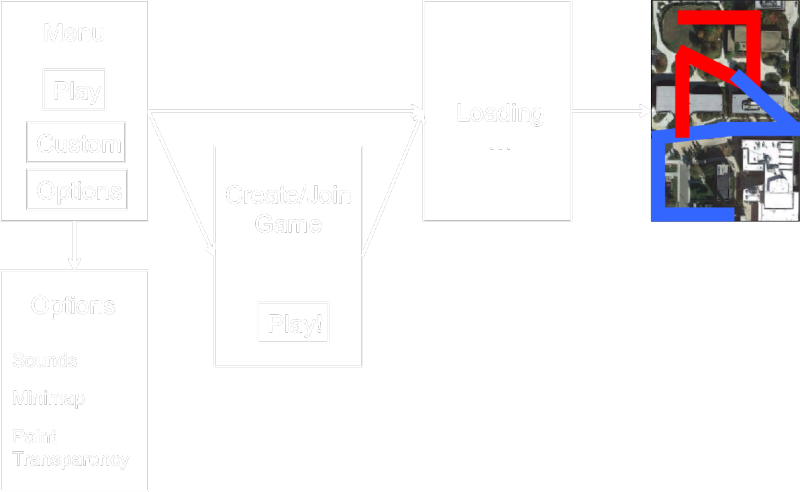
\includegraphics[width=.75\textwidth]{./assets/storyboard.png}
            \caption{The Main Storyboard}
        \end{figure}

    \end{frame}


    \begin{frame}
        \frametitle{Design}
        \framesubtitle{The Architecture}

        \begin{figure}[!ht]
            \centering
            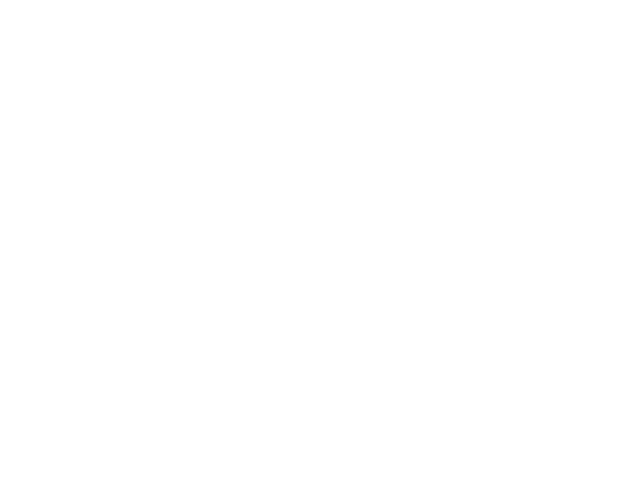
\includegraphics[width=.75\textwidth]{./assets/model.png}
            \caption{The Game Model}
        \end{figure}

    \end{frame}


    \begin{frame}
        \frametitle{Lessons Learned}
        \framesubtitle{Mistakes Were Made. Lessons Were Learned.}

        What worked:

        \begin{itemize}
            \item Breaking up into server, Android, and iOS teams --- distributes workload well
            \item Swift instead of Objective-C for iOS --- safer to develop in
        \end{itemize}

        What didn't work:

        \begin{itemize}
            \item Difficult to get the map functionality we want with \syntaxbox{MKMapView} on iOS
        \end{itemize}
    \end{frame}

    \hugeslide{Demo}
\end{darkframes}
\end{document}
